%% ISAE-SUPAERO report template for research projects 
%% V1.0
%% 2016/04/14
%% by Damien Roque
%% See http://personnel.isae.fr/damien-roque


%% This template is based on bare_conf.tex
%% V1.4b
%% 2015/08/26
%% by Michael Shell

%%*************************************************************************
%% Legal Notice:
%% This code is offered as-is without any warranty either expressed or
%% implied; without even the implied warranty of MERCHANTABILITY or
%% FITNESS FOR A PARTICULAR PURPOSE! 
%% User assumes all risk.
%% In no event shall the IEEE or any contributor to this code be liable for
%% any damages or losses, including, but not limited to, incidental,
%% consequential, or any other damages, resulting from the use or misuse
%% of any information contained here.
%%
%% All comments are the opinions of their respective authors and are not
%% necessarily endorsed by the IEEE.
%%
%% This work is distributed under the LaTeX Project Public License (LPPL)
%% ( http://www.latex-project.org/ ) version 1.3, and may be freely used,
%% distributed and modified. A copy of the LPPL, version 1.3, is included
%% in the base LaTeX documentation of all distributions of LaTeX released
%% 2003/12/01 or later.
%% Retain all contribution notices and credits.
%% ** Modified files should be clearly indicated as such, including  **
%% ** renaming them and changing author support contact information. **
%%*************************************************************************

\documentclass[conference]{IEEEtran}

\usepackage[utf8]{inputenc}
\usepackage{ifthen}
\usepackage{cite}
\usepackage{booktabs}
\usepackage{tabu} 
\usepackage[pdftex]{graphicx}
\graphicspath{{images/}}
\usepackage{tikz,filecontents}
\usetikzlibrary{shapes,arrows,shadings,patterns}
\usepackage{pgfplots}
\pgfplotsset{compat=newest}
\pgfplotsset{plot coordinates/math parser=false}
\newlength\figureheight
\newlength\figurewidth
\bibliographystyle{unsrt}

\usepackage{amsfonts}
\usepackage[cmex10]{amsmath}
\usepackage{multirow}
\usepackage{graphicx}

% Examples of several macros
\newcommand*{\SET}[1]{\ensuremath{\boldsymbol{#1}}}
\newcommand*{\VEC}[1]{\ensuremath{\boldsymbol{\mathrm{#1}}}}
\newcommand*{\FAM}[1]{\ensuremath{\mathrm{#1}}}
\newcommand*{\MAT}[1]{\ensuremath{\boldsymbol{\mathrm{#1}}}}
\newcommand*{\OP}[1]{\ensuremath{\mathrm{#1}}}
\newcommand*{\NORM}[1]{\ensuremath{\left\|#1\right\|}}
\newcommand*{\DPR}[2]{\ensuremath{\left \langle #1,#2 \right \rangle}}

\newtheorem{theorem}{Theorem}

\newcommand{\alert}[1]{\textcolor{red}{#1}}
\usepackage[caption=false,font=footnotesize]{subfig}
\usepackage{url}

% correct bad hyphenation here
\hyphenation{op-tical net-works semi-conduc-tor}

\begin{document}
%
% paper title
% Titles are generally capitalized except for words such as a, an, and, as,
% at, but, by, for, in, nor, of, on, or, the, to and up, which are usually
% not capitalized unless they are the first or last word of the title.
% Linebreaks \\ can be used within to get better formatting as desired.
% Do not put math or special symbols in the title.
\title{Gaussian Process for Surrogate Modelling: Application in Non-Linear Mechanics}

% for over three affiliations, or if they all won't fit within the width
% of the page, use this alternative format:
% 

\author{\IEEEauthorblockN{Tianyi LI\IEEEauthorrefmark{1},
% Student2\IEEEauthorrefmark{1},
Joseph MORLIER\IEEEauthorrefmark{2}, Simone CONIGLIO\IEEEauthorrefmark{3} and 
Pierre-jean BARJHUX\IEEEauthorrefmark{4}}

\IEEEauthorblockA{\IEEEauthorrefmark{1}Institut Supérieur de l'Aéronautique et de l'Espace (ISAE-SUPAERO), Université de Toulouse, 31055 Toulouse, FRANCE\\
Email: Tianyi.LI@student.isae-supaero.fr}
\IEEEauthorblockA{\IEEEauthorrefmark{2}Institut Supérieur de l'Aéronautique et de l'Espace (ISAE-SUPAERO), Université de Toulouse, 31055 Toulouse, FRANCE\\
Email: joseph.morlier@isae-supaero.fr}
\IEEEauthorblockA{\IEEEauthorrefmark{3}Institut Supérieur de l'Aéronautique et de l'Espace (ISAE-SUPAERO), Université de Toulouse, 31055 Toulouse, FRANCE\\
Email: simone.coniglio91@gmail.com}
\IEEEauthorblockA{\IEEEauthorrefmark{4}Institut Supérieur de l'Aéronautique et de l'Espace (ISAE-SUPAERO), Université de Toulouse, 31055 Toulouse, FRANCE\\
Email: pierre-jean.barjhoux@irt-saintexupery.com}
}


% \IEEEspecialpapernotice{(Bibliography report)}
\IEEEspecialpapernotice{(Final report)}


% make the title area
\maketitle

% As a general rule, do not put math, special symbols or citations
% in the abstract
\begin{abstract}
In engineering design problems, advanced simulations are time consuming and computationally expensive. As a cheap replacement of the expensive simulations, surrogate models have been widely accepted as an efficient tool of computational engineering design. Gaussian Process Regression (GPR) method is used in this article as a replacement of Finite Element Simulation to predict the maximum principle stress and its location of a non-linear model. The results show that GPR method can give accurate prediction of maximum principle stress and its location of a nonlinear model.

Keywords: Gaussian Process Regression; Surrogate Modelling; Non-Linear Mechanics; Finite Element Method; Maximum Principle Stress
\end{abstract}
\IEEEpeerreviewmaketitle

\section{Introduction}
\subsection{Motivation}
\label{sec:problem-statement}

% Describe the context of your project here. Prior work must be referenced and discussed 
Engineering design requires engineers to precise decisions out of numerous analysis. These engaged analysis could spend month time by dedicated teams. The 'Surrogate model' approach is proposed as an approximate model that can greatly reduce both time and cost in engineering design problems\cite{forrester2008engineering}.

%The core objective of surrogate modelling is to find a transformation function between the inputs and outputs.
Using part of the results obtained from simulations or experiments as a training set, a surrogate model is trained and built. The established model is then optimized and tested to find the best possible function explaining the data. Once the surrogate model is well established, it can be used to predict the output of new data\cite{chiplunkar2016sparse}.
% Further instructions can be found at \url{https://www.ieee.org/documents/ieeecitationref.pdf}.

\subsection{Problem statement}
\label{sec:problem-statement}
This project aims to construct a surrogate model to predict maximum principle stress and its location of a non-linear model. As shown in Figure 1, the life cycle of a simple non-linear component can be reduced to a linear combination of loads,$F_1$,$F_2$. The model is non linear due to contact with the red pin in the middle of the structure. Each load combination should be executed to analyze the life cycle due to the non-linearity. Since the Finite Element Analysis can be very expensive and the number of load combination can be of 5000 different loads, this approach can be prohibitive. As a replacement of finite element simulation,  surrogate models are constructed so as to bridge the gap between accuracy and complexity. 

% \begin{figure}[htp]
%   \centering
%   \setlength\figureheight{5cm}
%   \setlength\figurewidth{6cm}
%   \input{images/model.pdf}
%   \caption{An accurate caption should be written here}
% %   \label{tex:my-figure}
% \end{figure}
\begin{figure} 
\centering
\includegraphics[width=3.5in,height=2.4in]{model1.jpg}
\caption{Non-linear model of a small aircraft component}
\label{fig:graph}
\end{figure}

% Explain what are the main issues to be addressed in this project...
\section{Methods}
The type of surrogate model used in this project is Gaussain Process Regression (also called Kriging model), which is a subset of the Bayesian Inference algorithms. Before going into the principle of Gaussian Process, it is necessary to have a look at the Bayesian linear regression algorithm\cite{neal2012bayesian}. 
\subsection{Bayesian Linear Regression}
Suppose that we have already got a training set with observations (or outputs):
$y=(y(x_1),...,y(x_i),...,y(x_N))^T$ 
evaluated at inputs $X=(x_1,...,x_i,...,x_N)^T$. Our goal is to predict $y(x_*)$ at a test input $x_*$.
The process of Bayesian linear regression consists of three steps: assuming a functional form of f (representation), minimizing the error between the observed outputs (y) and the predicted outputs f(x)(evaluation) and optimizing parameters of f (optimization). The function is written in terms of linear basis functions $\phi(x)=\left\{ 1,x \right\}^T$. 

\begin{equation}
%   \label{eq:tx}
  f(x)=\left\{ 1\quad x \right\} \left\{ w_0 \quad w_1 \right\}^T
\end{equation}

$w_0$,$w_1$ are the parameters of the function. The above equations can be combined to result in the likelihood $Pr[y|X,w]$.

\begin{equation}
%   \label{eq:tx}
  Pr[y|X,w]={\mathcal N} ( X^T \omega , \sigma_n^2 I_N )
\end{equation}

$Pr[y | X , w]$ is probability distribution of the outputs y at the inputs X. The ${\mathcal N} [\mu, \Sigma ] $ symbolizes a multi-variate Gaussian distribution with mean vector $\mu$ and covariance matrix $\sigma$. 

A prior is a probability distribution before looking at the observations. Since uncertainty about the mean function can be taken into account by adding an extra term to the covariance function, a zero mean Gaussian prior was put on weights.

\begin{equation}
%   \label{eq:tx}
  Pr[w]={\mathcal N} (0, \sigma_{prior})
\end{equation}

Once we have the prior distribution, Bayes rule was used to get a posterior distribution of parameters. Combining the equation 1, 2 and 3, the posterior distribution of weights can be derived:

\begin{equation}
%   \label{eq:tx}
  Pr[w|y,X]={\mathcal N} (\frac{1}{\delta_n^2}A^{-1}Xy , A^{-1})     
\end{equation}

In above equation, $A=\delta_n^{-2}XX^T+\sigma_prior^{-2}$. Then we can get the posterior distribution for function $f$ at test point $x_*$:

\begin{equation}
%   \label{eq:tx}
  Pr[f|x_*,X,y]={\mathcal N} (\frac{1}{\delta_n^2}x_* A^{-1}Xy , x_*^T A^{-1}x_*)     
\end{equation}

It is worth noting that in equation 5, the mean $\frac{1}{\delta_n^2}x_* A^{-1}Xy$ can be used as a prediction at the test point $x_*$ and variance $x_*^T A^{-1}x_*$ can be the confidence interval for the prediction\cite{mackay2003information}. 

\subsection{Gaussian Process Regression Principle}

Gaussian Process is a distribution over functions. Compared with Bayesian linear regression, GPs enable us to encode prior knowledge directly in the functional space.

A GP model can be completely parameterized by its mean and its covariance function before introducing training data. The mean function represents the trend of functions, while the covariance function defines the spatial dependency between input-points\cite{duvenaud2014automatic}\cite{wilson2014covariance}.

\begin{equation}
%   \label{eq:tx}
  Pr[f(x)] = GP(m(x),k(x_1,x_2))  
\end{equation}

$Pr(f(x))$ is probability distribution of function f at point x. The mean function m(x) is often assumed to be zero because uncertainty about the mean function can be taken into account by adding an extra term to the covariance function. In this way, the GP model can be completely parametrized by the covariance function. Therefor GP learning problem is exactly the problem of finding proper properties of the covariance function.

Once the prior is well defined, we wish to make use of the information of the training data-set. Same as Bayesian rules, a posterior is defined as the probability distribution after updating information of training data into prior distribution.

The measured outputs with noise can be written as:
\begin{equation}
%   \label{eq:tx}
  y(x) = f (x) + \varepsilon
\end{equation}

In equation 7, $\varepsilon$ represents an independent random noise sampled from $\mathcal{N}(0,\sigma_n^2)$. We can thus obtain its prior GP:

\begin{equation}
%   \label{eq:tx}
  Pr[y(x)] = GP(0,k(x_1,x_2)+\sigma_n^2 \delta_{x_1,x_2})  
\end{equation}

$\delta_{x_1,x_2}$ is a Kronecker delta function. According to above equations, the joint distribution of the training outputs $y(X)$ and true value $f(X)$ is shown below:

\begin{equation}
%   \label{eq:tx}
Pr\left[ \begin{array}{ccc}
y(x)\\
f(x_*) \\ 
\end{array} 
\right ]=\mathcal{N} (\left[ \begin{array}{ccc}
0\\
0 \\ 
\end{array} 
\right] ,\left[ \begin{array}{ccc}
K(X,X)+ \sigma_n^2 I_N & K(X,X_*)\\
K(X_*,X)& K(X_*,X_*)\\
\end{array} 
\right ] )
\end{equation}

The posterior distribution of $f(X_*)$ can be calculated as follows:
\begin{multline}
  Pr[f(x_*)|X_*,X,y(X)]=\\GP( K(X_*,X)(K(X,X)+ \sigma_n^2 I_N)^{-1} f(X), \\
  K(X_*,X_*)- K(X,X_*)(K(X,X)+ \sigma_n^2 I_N)^{-1} K(X,X_*))
\end{multline}

We can see from eqution 10 that the predictive mean is a linear combination of the observations and the predicted variance in not dependent on the observations $y$. Same as Bayesian rules, the mean here is a prediction at the test point and predicted variance can be used as an efficient method to track uncertainties arising from the prior assumption and observations\cite{shah2014student}.

\subsection{Covariance Functions}
As we mentioned before, the mean function is zero. Therefor the properties of functions under a GP are controlled by the functional form of the covariance and its hyper-parameters\cite{rasmussen2004gaussian}. In order to give a accurate prediction, functional form selection and  hyper-parameters optimization are very important.

\subsubsection{Covariance Functions} As most common used covariance functions, SE(squared exponentia) kernel, Matérn kernel and RQ(rational quadratic) kernel are used in this project.
\subsubsection*{Squared Exponential Kernel} 
\begin{equation}
  k_{SE}(d,\theta) =\theta_{amplitude}^2 exp(-\frac{d^2}{2\theta_{lengthscale}})
\end{equation}
\subsubsection*{Matérn Kernel} 
\begin{multline}
   k_{Matern}(\upsilon=\frac{3}{2},d,\theta) =\\ \theta_{amplitude}^2 (1+\frac{\sqrt[]{3}d}{\theta_{lengthscale}})exp(\frac{\sqrt[]{3}d}{\theta_{lengthscale}})
\end{multline}
\subsubsection*{Rational Quadratic Kernel} 
\begin{equation}
  k_{RQ}(\alpha,k,d) =(1+\frac{d^2}{2\alpha k^2})^{-\alpha}
\end{equation}
\subsubsection{Hyperparameters}
We can see from above equations that these covariance functions are specified by a set of parameters. In GP, they are called hyper-parameters. In this project, optimal hyper-parameters are found by calculating and maximizing the marginal likelihood\cite{mackay2003information}:
\begin{multline}
  log (Pr[y|X,\theta]) = -\frac{1}{2} y^T[K(X,X)+\sigma_n^2 I_N]^{-1}y \\ - log|K(X,X)+ \sigma_n^2 I_N|- \frac{N}{2}log(2\pi)
\end{multline}
There are three terms in marginal likelihood\cite{rasmussen2004gaussian}: a data-fit term
  $-\frac{1}{2} y^T[K(X,X)+\sigma_n^2 I_N]^{-1}y$, a model complexity term $ - log|K(X,X)+ \sigma_n^2 I_N|$, and a normalization term $-\frac{N}{2}log(2\pi)$.
 
The optimal hyper-parameters we get from maximizing the marginal likelihood are the local maximums. In order to obtain global optimum, Leave-One-Out-Cross-Validation will be used in this project\cite{le2013multi}\cite{bouhlel2016optimisation}.

\subsection{Error Analysis Method}
\subsubsection{Leave-One-Out-Cross-Validation}
As mentioned above, Leave-One-Out-Cross-Validation is used to find the global optimum of hyper-parameters. The main idea of CV is to split the experimental design set into two disjoint sets, one is used for training and the other one is used to testing the surrogate model. Leave-One-Out (LOO) is a special case of CV where test sets are obtained by removing one observation at-a-time.
\subsubsection{Error Measurement Method}
In order to test the performance of the established surrogate model, we need to measure the error between the observed outputs and the predicted outputs. Root-mean-square Error($RMSE$) and $R^2$ are used in this manuscript.
\subsubsection*{Root-mean-square Error}
\begin{equation}
  RMSE=\sqrt[]{\frac{\sum_{i=1}^{n}(Y_i-\hat{Y}_i)^2}{n}}
\end{equation}
\subsubsection*{$R^2$ Error}
\begin{equation}
 R^2=1-\frac{\sum_{i=1}^{n}(Y_i-\hat{Y}_i)^2}{\sum_{i=1}^{n}(Y_i-\overline{Y}_i)^2}
\end{equation}
In above equations, $Y_i$ is observed outputs, $\hat{Y}_i$ is predicted output and $\overline{Y}_i$ is the mean of observed outputs. It is worth noting that our prediction is more accurate when the $RMSE$ is closer to zero. For $R^2$, the closer its value is to one, the more accurate our prediction is.


% Kriging method\cite{forrester2008engineering} supposes that responses of data points are correlated and its values depend on the ‘distance’ between input points. 
% \begin{equation}
%   \label{eq:tx}
%   cor[Y(x^{(i)},)Y(x^{(l)}] = exp(-\sum_{j=1}^{K-1}\theta_j | x^{(i)}_{j} -x^{(l)}_{j}|^{p_j})
% %   \sum_{k=0}^{K-1} \sum_{m=0}^{M-1} c_{k,m} g[l-mN] e^{j2\pi \frac{k}{K}l}, \quad l \in \SET{Z}.
% \end{equation}
% ~~~~Equation 1 indicates that the correlation of the responses in two points $x^{(i)}$ , $x^{(l)}$ 
% depend on the absolute distance between the
% sample points and the parameters $\theta_j$ and $p_j$. Kriging method also supposes that the predicted output is a linear combination of observed responses. $w_i$ are the weights and its reflect the structural "proximity" of samples to the estimation location. 
% \begin{equation}
%   \label{eq:tx}
%  \hat{y}(x)= \sum_{i=0}^{n} w_{i} y_{i}
% \end{equation}
% ~~~C E Rasmussen et. al.\cite{rasmussen2004gaussian} give another understanding of Gaussian process. 
% It starts with the prior distribution over functions specified by a particular Gaussian process.This prior is taken to represent our prior beliefs over the kinds of functions we expect to observe, before seeing any data. Samples from a function will be normally distributed, where the covariance between any two samples is the covariance function (or kernel) of the Gaussian process evaluated at the spatial location of two points. A set of values is then observed, each value associated with a spatial location. Now, a new value can be predicted at any new spatial location, by combining the Gaussian prior with a Gaussian likelihood function for each of the observed values. The resulting posterior distribution is also Gaussian, with a mean and covariance that can be simply computed from.

% \subsection{Applications in solving engineering problems}
% H.Xu et. al.\cite{xu2016towards} have proposed a supervised learning-enhanced cokriging method to solve multi-material structural design problems. The proposed method is compared with several existing mixed-variable Surrogate model methods to understand their pros and cons. These methods include Neural Network (NN) regression, Classification and Regression Tree (CART) and Gaussian Process (GP). By applying all these methods to optimize material selection and structure design of coil spring, Gaussian Process Regression is found to have a better accuracy and robustness comparing to other surrogate model methods when there is a small number of training points.

% A.Chiplunkar et.al.\cite{chiplunkar2017operational,chiplunkar2016sparse,chiplunkar2016adding} have proposed to build better Gaussian Process (GP) regression models by integrating the prior knowledge of Aircraft design with experimental data. For example, by using spectral mixture kernels, surrogates models are built for structural dynamic experiments and dynamic parameters such as modal frequency are automatically identified. Relationships between multiple outputs and two main methods of scaling Gaussian Process samples are also discussed in their article.

% S.Suram et.al.\cite{suram2008proper} have constructed a reduced order model for a hydraulic mixing nozzle using proper orthogonal decomposition (single value decomposition). 
% Flow structures are compared for the original and optimized shape nozzles to study the effect of changing the nozzle’s shape on the flow characteristics. Inspired by their study, single value decomposition can also be used in our project to get the reduced order model and reduce the code.


 
\section{Modeling process}
GPR models are first constructed to predict the maximum principle stress for each load combination. We then wish to give the prediction of the location of maximum stress. All the code is written in the basis of the code library provided in the book\cite{rasmussen2004gaussian} of C.E.Rasmussen
\subsection{Sampling Design}
As shown in Figure 2, two different sampling plans are used in this project.

\begin{figure} 
\centering
\includegraphics[width=3.8 in,height=2.7in]{sampling1.png}
\caption{Sampling plan}
\label{fig:graph}
\end{figure}

For sampling plan 1, seven different values are evenly taken from $[-1000,1000]$ for both $F1$ and $F2$. So there are 49 different load combination in total. We then obtain the maximum principle stress and its location for each load by ABAQUS simulation. Sampling plan 2 are obtained by evenly taking 11 values for both $F1$ and $F2$. Same as plan 1, their maximum principle stress and locations of maximums are also simulated by ABAQUS.
\subsection{Maximum Principle Stress}
\subsubsection{Hyper-parameter Optimization} Only the sampling plan 1 is used in predicting maximum stress. In order to build our surrogate model, we first determine inputs and outputs in the problem of predicting the maximum principle stress.
\begin{figure} 
\centering
\includegraphics[width=2 in,height=0.8 in]{IO2-1.png}
\caption{Input-Output for Maximum Prediction}
\label{fig:graph}
\end{figure}
As shown in Figure 3, this is a multiple inputs($F_1$ and $F_2$) with single output($\sigma_{max}$) GPR problem. We first select an empty mean function and a SE covariance function as prior information. Before predicting in the new data, we need to find the optimal hyper-parameters. As mentioned in third section, LOO-Cross-Validation is used here to find the global optimum. 

\subsubsection{Prediction in New Data} Once our surrogate model is well constructed and optimized, we wish to predict the maximum principle stress for new load combinations. 49 different loads and their corresponding maximum stress in sampling plan 1 are used as training set. 14 randomly generated loads and their corresponding maximum stress are used as testing set. 

\subsubsection{Comparison Between Different Covariance Functions} The prediction of maximum stress for new load combinations are also given in RQ and Matérn covariance function. Different surrogate models are constructed using different covariance functions. 

\subsection{Location of Maximum Principle Stress}
Unlike the prediction of maximum principle stress, the GPR learning of its location is a multiple outputs problem(shown in Figure 4).

\begin{figure} 
\centering
\includegraphics[width=2 in,height=0.8 in]{IO2-2.png}
\caption{Input-Output for Maximum Prediction}
\label{fig:graph}
\end{figure}

\subsubsection{Training X Coordinate and Y Coordinate Separately} Without considering the relationship between the x and y coordinates, we first divide this problem into two single-output training problem. The x and y coordinates are trained as output separately and two surrogates models are constructed.  

\subsubsection{Training in Polar Coordinate} As loads are applied on the center of the model, the maximum stress occur in the inner circle(Figure 5). In this way, this problem could be simplified into a single output problem by changing Cartesian coordinate(x,y) into Polar coordinate($\phi$,r=cste).

\begin{figure} 
\centering
\includegraphics[width=3 in,height=1.8 in]{innercycle.png}
\caption{Location of Maximum Stress}
\label{fig:graph}
\end{figure}

\subsubsection{Training with 121 training samples } Finally, Sampling plan 2 with more sample points is used as training set to predict the position of the maximum stress.

\section{Results}
\subsection{Maximum Principle Stress Prediction}
\subsubsection{Hyper-parameter Optimization}
Before predicting maximum stress for new loads, LOO-Cross-Validation is used to get the global optimal hyper-parameters. The optimum hyper-parameters found in SE kernel are $[d=7.17~~ \theta=3.50]$ (equation 11).
\subsubsection{Prediction in New Data}
Once our surrogate model is well constructed, the predictive accuracy is tested. 

\begin{figure} 
\centering
\includegraphics[width=3.4 in,height=2.5 in]{14-1.png}
\caption{Evaluation of GPR Model}
\label{fig:graph}
\end{figure}

In figure 6, x-axis and y-axis represent inputs $F_1$ and $F_2$, respectively. The z-axis represents the maximum principle stress. The black dots represent the training data, the red dots represent the predicted output, and the blue dots represent the observed output. We can see from Figure 6 that the red dots and blue dots are either very close or coincident. Therefore, intuitively our GP model can give accurate predictions for maximum principle stress.

\begin{figure} 
\centering
\includegraphics[width=3.4 in,height=2.5 in]{14-2.png}
\caption{Fitted line}
\label{fig:graph}
\end{figure}

As shown in figure 7, the x-axis represents the predicted output and the y-axis represents the observed output. Therefore, the position of points on the graph can represent the difference between the observed value and the predicted value. When the points are distributed along the line $y=x$, it means that the predictions are close to the observations. However, when the points are distributed around the x-axis and y-axis, our GPR model fails to give accurate predictions. 

A straight line is fitted according to the points in the figure 7. The equation for this line is $y =    1.01 x-0.41$. As its slope is approximately equal to 1 and the intercept is close to 0, it can be assumed that the prediction results are close to the observations. In addition, the RMSE between the predicted value and the true value is 0.5431, which also indicates that our GP model has a very high prediction accuracy.


\subsubsection{Comparison Between Different Covariance Functions}
SE kernel, RQ kernel, Matérn kernel and their combinations are also used as covariance functions to predict the maximum stress. We wish to explore the influence of the covariance function on the prediction results. The results are shown in table 1. RMSE and $R^2$ error are calculated for each covariance function. At the same time, the corresponding code running time is also given. The code running time is taken as the average of ten runs and computations were done on a Intel Core i5-2410M CPU 3.1 GHz.

We first focus on three simple covariance function. It is not difficult to see that their corresponding learning time is almost the same, while matérn kernel has the highest prediction accuracy, with a RMSE of 0.6385 and a $R^2$ of 0.9855. On the whole, the combined covariance functions have higher prediction accuracy than single kernel functions, but their running time also increases. The combination of SE, RQ and Matérn has the most accurate prediction and the longest running time. Therefore, if there are only tens of samples in training set, the combination of SE, RQ and Matérn can be used to get the best performance. But when there are hundreds of samples in training set, it is more appropriate to use a simpler covariance function to improve training efficiency.

\begin{table*}[t]
  \renewcommand{\arraystretch}{1.5}
  \caption{ERROR ANALYSIS}
  \label{tab:my-table}
  \centering
%  \begin{tabu}{lllllllr}
 \begin{tabu} to 0.8\linewidth {lccccccc}
\hline
% \multicolumn{2}{c}{Item} \\
\cline{1-8}
Error     &$SE$    &$RQ$     &$Matern$  &$SE+RQ$  &$SE+Matern$   &$RQ+Matern$ &$SE+RQ + Matern$\\
\hline
RMSE      &0.9582  &0.7179   &0.6285    &0.6250   &0.6176        &0.6174      &0.5431\\
$R^2$     &0.9659  &0.9809   &0.9853    &0.9855   &0.9858        &0.9858      &0.9890\\
\cline{1-8}
Time Cost/s &0.26    &0.32     &0.32      &0.53     &0.56          &0.58        &0.80\\
\hline
\end{tabu}
 \end{table*}

\subsection{Maximum Principle Stress Location Prediction}
After predicting the maximum stress, we then construct surrogate models to predict its location.
\subsubsection{Training X Coordinate and Y Coordinate Separately}
The X coordinate and Y coordinate are first trained as output separately. Same principle as figure 7, Figures 8 and 9 show the fitting curves for the x and y coordinates, respectively. The equations of their fitted lines are $y = 2.5x + 27.8$ and $y = 0.93x - 0.74$. Besides, the RMSE of X coordinate is 5.18 and RMSE of Y coordinate is 3.65. 

It is not difficult to see that the predicted results are far from what we expected. There are two possible reasons. First of all, the relationship between the x-coordinate and the y-coordinate of the maximum location is not considered. As discussed above, the maximum principle stress occurs on the inner ring of our model. Moreover, 49 training samples are too few to predict the location of maximum principle stress. 



\begin{figure} 
\centering
\includegraphics[width=3.4 in,height=2.5 in]{XY_x.jpg}
\caption{Fitted Line for X Coordinate When Training X Y Separately}
\includegraphics[width=3.4 in,height=2.5 in]{XY_y.jpg}
\caption{Fitted Line for Y Coordinate When Training X Y Separately}
\label{fig:graph}
\end{figure}

% \begin{figure} 
% \centering
% \includegraphics[width=3.4 in,height=2.5 in]{XY_y.jpg}
% \caption{Fitted Line for Y Coordinate When Training X Y Separately}
% \label{fig:graph}
% \end{figure}

\subsubsection{Training in Polar Coordinate}
As explained before, we can simplify the problem by using angle in Polar coordinate as the only output. Once we obtain the predicted angle, we convert it to the Cartesian coordinate and compare with observations.

\begin{figure} 
\centering
\includegraphics[width=3.4 in,height=2.5 in]{49_x.jpg}
\caption{Fitted Line for X Coordinate When Training in Polar Coordinate}
\includegraphics[width=3.4 in,height=2.5 in]{49_y.jpg}
\caption{Fitted Line for Y Coordinate When Training in Polar Coordinate}
\label{fig:graph}
\end{figure}

Figures 10 and 11 show the fitting curves for the x and y coordinates, respectively. The equations of their fitted lines are $y = 0.52 x -9.9$ and $y = 0.70x + 0.02$. Besides, the RMSE of X coordinate is 5.61 and RMSE of Y coordinate is 3.90. Although the problem is simplified and the running time is halved, the accuracy of the prediction does not improve. In this case, the number of training samples may be the decisive factor in determining the prediction accuracy.

\subsubsection{Training with 121 training samples }

Number of training samples increases from 49 to 121 by using Sample Plan 2. The results are shown in figure 12 and figure 13. The equations of fitted lines for the x and y coordinates are $y =0.88 x -3$ and $y = 0.80x $, respectively.  The RMSE of X coordinate is 3.7 and RMSE of Y coordinate is 3.0. By increasing the number of training samples, the prediction output gets closer to the observation output. Unlike the prediction of the maximum principle stress, more training data are needed to establish the GPR model to predict its location.

\begin{figure} 
\centering
\includegraphics[width=3.4 in,height=2.5 in]{121_x.jpg}
\caption{Fitted Line for X Coordinate When Training in Polar Coordinate}
\includegraphics[width=3.4 in,height=2.5 in]{121_y.jpg}
\caption{Fitted Line for Y Coordinate When Training in Polar Coordinate}
\label{fig:graph}
\end{figure}

\section{Conclusion}
Gaussian Process is a very important machine-learning method. It enable us to encode prior information directly in the functional space. GPs not only gives the prediction, but also the corresponding uncertainty information.

Gaussian Process Regression is a very efficient tool to predict maximum stress for a non-linear model. After learning with 49 training samples and testing with 14 randomly generated samples, the RMSE between the observations and predictions is calculated as 0.5431 and the line equation is $y=1.01x-0.41$. These results show that GPR can give accurate predictions in estimating maximum principle stress.

The covariance function has a significant influence on the prediction result. Combined covariance functions have higher accuracy than simple covariance functions, but their running time also increases.

Unlike the prediction of maximum stress, the prediction of its location requires more training samples. The prediction accuracy improves significantly after increasing training data from 49 to 121. 

\section{Future Work}

\subsubsection{Changing Sampling Method}
Latin Hypercube Sampling can be used and replace Sampling Plan 1 and 2.

\subsubsection{Using Proper Orthogonal Decomposition(POD) with large number of samples}
We can increase the number of training samples to several hundreds when predicting the location of maximum principle stress. POD can be used to simplify large sample size problems.

\subsubsection{Infill Criteria}
It is possible to enhance the accuracy of the model using infill points, in addition to the initial sampling plan. For example, we can find the point with maximum variance et add a training sample at this point.
 

% The whole project planning can be summarized as follows: 

% 1. Read the ABAQUS output information to MATLAB. 

% 2. Construct a surrogate model to predict the maximum principle stress for each load combination.

% $\bullet$ Input: Loads: $F_x$,$F_y$.

% $\bullet$  Output: Maximum Principle Stress $\sigma_{max}$

% 3. Optimize the surrogate model to predict the maximum principle stress and its position for each load combination 

% $\bullet$ Input: Node coordinates: $x$,$y$, Loads: $F_x$,$F_y$.

% $\bullet$ Output: Max Principle Stress $\sigma_{max}$, Position: $x_{max}$, $y_{max}$.


% 4. Construct a surrogate model to predict the principle stress distribution on each node for each load combination.

% $\bullet$ Input: Node coordinates: $x$,$y$, Loads: $F_x$,$F_y$.

% $\bullet$ Output: Principle Stress on each node: $\sigma$.

% 5. Use singular value decomposition (SVD) based learning algorithm to reduce the code.
% \subsection{First Result}
% Until now I have finished the first step of my project: writing the Matlab code to read the ABAQUS output information to MATLAB. The principle stress $\sigma$ on each node with its coordinate $x$,$y$ for each load combination have been read and storied in Matlab matrix.

% Equations can be used:
% \begin{equation}
%   \label{eq:tx}
%   s[l] = \sum_{k=0}^{K-1} \sum_{m=0}^{M-1} c_{k,m} g[l-mN] e^{j2\pi \frac{k}{K}l}, \quad l \in \SET{Z}.
% \end{equation}
% Do not forget to define each variable and symbol...

% Figures should be included as floats and properly referenced in the text (Fig. \ref{fig:my-figure}). The same rule applies for tables (Tab. \ref{tab:my-table})

% \begin{figure}[htp]
%   \centering
%   \setlength\figureheight{5cm}
%   \setlength\figurewidth{6cm}
%   % This file was created by matlab2tikz.
% Minimal pgfplots version: 1.3
%
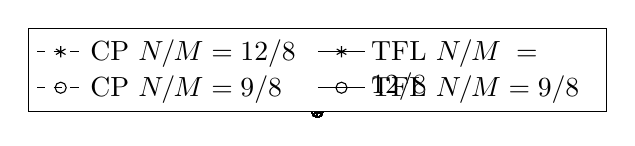
\begin{tikzpicture}

\begin{axis}[%
width=\figurewidth,
height=\figureheight,
at={(0\figurewidth,0\figureheight)},
scale only axis,
separate axis lines,
every outer x axis line/.append style={black},
every x tick label/.append style={font=\color{black}},
xmin=0,
xmax=600,
xlabel={$l_0$},
xmajorgrids,
every outer y axis line/.append style={black},
every y tick label/.append style={font=\color{black}},
ymin=15,
ymax=20,
ylabel={Gain [dB]},
ymajorgrids,
%legend style={legend cell align=left,align=left,draw=black}
legend columns=2,
legend style={text width=8em,legend cell align=left,align=left,draw=black,at={(0.5,1.05)}, anchor=south}
]
\addplot [color=black,dashed,mark=asterisk,mark options={solid}]
  table[row sep=crcr]{%
0	18.2390874094432\\
32	18.2390874094432\\
64	18.2390874094432\\
96	18.2390874094432\\
128	18.2390874094432\\
160	18.2390874094432\\
192	18.2390874094432\\
224	18.2390874094432\\
256	18.2390874094432\\
288	18.2390874094432\\
320	18.2390874094432\\
352	18.2390874094432\\
384	18.2390874094432\\
416	18.2390874094432\\
448	18.2390874094432\\
480	18.2390874094432\\
512	18.2306327719818\\
544	17.9540613758438\\
576	17.6689966399943\\
};
\addlegendentry{CP $N/M=12/8$};

\addplot [color=black,solid,mark=asterisk,mark options={solid}]
  table[row sep=crcr]{%
0	19.9999796047627\\
32	19.9782454264971\\
64	19.9172921503127\\
96	19.819523640774\\
128	19.6869764401989\\
160	19.5221481900787\\
192	19.3264690408576\\
224	19.1028168133025\\
256	18.8524145582619\\
288	18.5769651836831\\
320	18.2797229467138\\
352	17.9588025753321\\
384	17.6198925633198\\
416	17.2597387528296\\
448	16.8807108312221\\
480	16.4832729985219\\
512	16.0669779302672\\
544	15.6289248101717\\
576	15.1692321920288\\
};
\addlegendentry{TFL $N/M=12/8$};

\addplot [color=black,dashed,mark=o,mark options={solid}]
  table[row sep=crcr]{%
0	19.4884747755262\\
32	19.4884747755262\\
64	19.4884747755262\\
96	19.4884747755262\\
128	19.4800794761447\\
160	19.2039363265844\\
192	18.9194155478691\\
224	18.6243664611488\\
256	18.3193439905467\\
288	18.0035198444507\\
320	17.6753775333409\\
352	17.3329477537639\\
384	16.9775142144053\\
416	16.6049465654203\\
448	16.2214034199632\\
480	15.8132879400791\\
512	15.3931020845481\\
544	14.9429381335956\\
576	14.4724841527662\\
};
\addlegendentry{CP $N/M=9/8$};

\addplot [color=black,solid,mark=o,mark options={solid}]
  table[row sep=crcr]{%
0	19.9999188401472\\
32	19.9198402053393\\
64	19.7226565216249\\
96	19.4581952942028\\
128	19.165296513424\\
160	18.8621944283946\\
192	18.5462056497272\\
224	18.2187733804306\\
256	17.8809942229679\\
288	17.5256445475455\\
320	17.1574123511579\\
352	16.769914008492\\
384	16.3698267920046\\
416	15.9497164928657\\
448	15.5024807138218\\
480	15.0375569039195\\
512	14.5394847970002\\
544	14.0174757064722\\
576	13.4597208888491\\
};
\addlegendentry{TFL $N/M=9/8$};

\end{axis}
\end{tikzpicture}%
%   \caption{An accurate caption should be written here}
%   \label{fig:my-figure}
% \end{figure}

% \begin{table}[htp!]
%   \renewcommand{\arraystretch}{1.5}
%   \caption{ERROR ANALYSIS}
%   \label{tab:my-table}
%   \centering
%   \begin{tabular}{|c|c|c|c|c|c|c|c|}
%     \hline
%     Error & $SE$ & $RQ$ & $Matern$ & $SE+RQ$ & $SE+Matern$& $RQ+Matern$ & $SE+RQ + Matern$\\
%     \hline
%     RMSE & $0.2566N$ & $2.12/M$ & $0.2263$ & $0.1226$ & $2.12/M$ & $2.12/M$ & $2.12/M$\\
%     \hline
%     MAPE & $0.2617N$ & $1.44/M$ & $0.1715$ & $0.1874$ & $2.12/M$ & $2.12/M$ & $2.12/M$\\
%     \hline
% %     NR-TFL & $0.2580N$ & $0.68/M$ & $0.1839$ & $0.4047$\\
% %     \hline
%   \end{tabular}
% \end{table}

 
% \begin{table}[htbp]
%  \caption{\label{tab:test}}
%  \begin{tabular}{lcl}
%   \toprule
%   。。 & 。。 & 。。 \\
%   \midrule
%  。。 & 。。 & 。。 \\
%  。。 & 。。 & 。。 \\
%  。。 & 。。 & 。。 \\
%   \bottomrule
%  \end{tabular}
% \end{table}

% Optional section
\section*{Acknowledgment}
I would like to thank my tutor Dr. Joseph Morlier, who gave me this opportunity to work on this project and also help me in the the academic side. My thanks also go to Dr. Simone Coniglio, who has presented the whole subject of this project to me and has told me how to finish my work step by step. Last but not least, I would like to express thanks to Dr. Pierre-jean Barjhoux with his kindly help with my questions in Matlab.

\bibliographystyle{plain}
\bibliography{references}

\end{document}


